%% FEUP THESIS STYLE for LaTeX2e
%% how to use feupteses (portuguese version)
%%
%% FEUP, JCL & JCF, 31 Jul 2012
%%
%% PLEASE send improvements to jlopes at fe.up.pt and to jcf at fe.up.pt
%%

%%========================================
%% Commands: pdflatex tese
%%           bibtex tese
%%           makeindex tese (only if creating an index)
%%           pdflatex tese
%% Alternative:
%%          latexmk -pdf tese.tex
%%========================================

%% 2021-07-20: One-sided output by default
\documentclass[11pt,a4paper]{report}
%% For two-sided printing (for dead-tree output) comment previous line
%% and uncomment the next line
%% \documentclass[11pt,a4paper,twoside,openright]{report}

%% For iso-8859-1 (latin1), comment next line and uncomment the second line
\usepackage[utf8]{inputenc}
%\usepackage[latin1]{inputenc}

%% Portuguese version

%% MEIC options
%\usepackage[portugues,meic]{feupteses}
%\usepackage[portugues,meic,juri]{feupteses}
%\usepackage[portugues,meic,final]{feupteses}
%\usepackage[portugues,meic,final,onpaper]{feupteses}

%% MEEC options
%\usepackage[portugues,meec]{feupteses}
%\usepackage[portugues,meec,juri]{feupteses}
%\usepackage[portugues,meec,final]{feupteses}
%\usepackage[portugues,meec,final,onpaper]{feupteses}

%% For other degrees
\usepackage[portugues]{feupteses} % you must define the degree bellow

%% Options: 
%% - portugues: titles, etc in portuguese
%% - onpaper: links are not shown (for paper versions)
%% - backrefs: include back references from bibliography to citation place

%% Uncomment to create an index (at the end of the document)
%\makeindex

%% Path to the figures directory
%% TIP: use folder ``figures'' to keep all your figures
\graphicspath{{figures/}}

%%----------------------------------------
%% TIP: if you want to define more macros, use an external file to keep them
\usepackage{color}
\usepackage{listings}
\lstset{ %
language=C++,                % choose the language of the code
basicstyle=\footnotesize,       % the size of the fonts that are used for the code
numbers=left,                   % where to put the line-numbers
numberstyle=\footnotesize,      % the size of the fonts that are used for the line-numbers
stepnumber=1,                   % the step between two line-numbers. If it is 1 each line will be numbered
numbersep=5pt,                  % how far the line-numbers are from the code
backgroundcolor=\color{white},  % choose the background color. You must add \usepackage{color}
showspaces=false,               % show spaces adding particular underscores
showstringspaces=false,         % underline spaces within strings
showtabs=false,                 % show tabs within strings adding particular underscores
frame=single,           % adds a frame around the code
tabsize=2,          % sets default tabsize to 2 spaces
captionpos=b,           % sets the caption-position to bottom
breaklines=true,        % sets automatic line breaking
breakatwhitespace=false,    % sets if automatic breaks should only happen at whitespace
escapeinside={\%*}{*)}          % if you want to add a comment within your code
}

\def\lstlistlistingname{List of Code}

% format
\newcommand{\class}[1]{{\normalfont\slshape #1\/}}

% entities
\newcommand{\IPCA}{Instituto Politécnico do Cávado e do Ave}

\newcommand{\svg}{\class{SVG}}
\newcommand{\scada}{\class{SCADA}}
\newcommand{\scadadms}{\class{SCADA/DMS}}


%%----------------------------------------

%%========================================
%% Start of document
%%========================================
\begin{document}

%%----------------------------------------
%% Information about the work
%%----------------------------------------
\title{Título da Dissertação}
\author{Nome do Autor}

%% Comment next line if not necessary for degree name
\degree{Programa Doutoral em Engenharia Informática}

%% Uncomment next line for date of submission
%\thesisdate{31 de julho de 2008}

%% Comment next line for copyright text if not used
\copyrightnotice{Nome do Autor, 2008}

\supervisor{Orientador}{Nome do Orientador}

%% Uncomment next line if necessary
%\supervisor{Co-orientador}{Nome de Outro Orientador}

%% Uncomment committee stuff in the final version if used
%\committeetext{Aprovado em provas públicas pelo Júri:}
%\committeemember{Presidente}{Nome do presidente do júri}
%\committeemember{Arguente}{Nome do arguente do júri}
%\committeemember{Vogal}{Nome do vogal do júri}

%% Uncomment signature line in the final on paper version if used
%\signature

%% Specify cover logo (in folder ``figures'')
\logo{uporto-feup.pdf}
 
%% Uncomment next line for additional text below the author's name (front page)
%\additionalfronttext{Preparação da Dissertação}

%%----------------------------------------
%% Preliminary materials
%%----------------------------------------

% remove unnecessary \include{} commands
\begin{Prolog}
  
\chapter*{Abstract}
%\addcontentsline{toc}{chapter}{Abstract}

This report serves as a guidance to the project of "Programação Imperativa", of the 1st year of IPCA's class "Engenharia de Sistemas Informáticos". % the abstract
  \chapter*{Agradecimentos}
%\addcontentsline{toc}{chapter}{Agradecimentos}

Gostaria de agradecer aos professores Óscar Ribeiro e João Carlos Silva pela oportunidade de realizar a melhoria de nota.

\vspace{10mm}
\flushleft{Bruna Macieira}
  % the acknowledgments
  \cleardoublepage
\thispagestyle{plain}

\vspace*{8cm}

\begin{flushright}
   \textsl{``You should be glad that bridge fell down. \\
           I was planning to build thirteen more to that same design''} \\
\vspace*{1.5cm}
           Isambard Kingdom Brunel
\end{flushright}
    % initial quotation if desired
  \cleardoublepage
  \pdfbookmark[0]{Conteúdo}{contents}
  \tableofcontents
  \cleardoublepage
  \pdfbookmark[0]{Lista de Figuras}{figures}
  \listoffigures
  \cleardoublepage
  \pdfbookmark[0]{Lista de Tabelas}{tables}
  \listoftables
  \chapter*{Abreviações e símbolos}
%\addcontentsline{toc}{chapter}{Abbreviations}
\chaptermark{Abbreviations and symbols}

\begin{flushleft}
\begin{tabular}{l p{0.8\linewidth}}
    IPCA      & Instituto Politécnico do Cávado e do Ave - (Polytechnic Institute of Cávado and Ave)\\
\end{tabular}
\end{flushleft}

  % the list of abbreviations used
\end{Prolog}

%%----------------------------------------
%% Body
%%----------------------------------------

\StartBody

%% TIP: use a separate file for each chapter
\chapter{Introdução} \label{chap:intro}

Este projeto foi realizado no âmbito das disciplinas "Laboratórios de Informática" e "Programação Imperativa".

\section{Contextualização} \label{sec:context}

O âmbito deste trabalho é criar um documento que sirva de suporte para o projeto realizado na Unidade curricular "Programação Imperativa". 
\chapter{Resolução} \label{chap:sota}

 O seguinte projeto é composto por 8 questões, sendo a primeira composta por 3 alíneas. 

 Alguns dos problemas propostos consistiam em:

\begin{itemize}
	\item carregar ficheiros de texto
	\item listagem de informação
	\item cálculo de determinadas fórmulas
	\item gerar tabelas
	\item gerar tabelas
	\item exportar tabelas para ficheiros binários
\end{itemize}

\section{Resolução}

Para a sua resolução, foi criado o "Main.h", onde seriam criadas as estruturas necessárias ao problema, cada uma referente a cada ficheiro de textos que já havia sido guardado, assim como as chamadas de todos os exercícios que seriam então criados. Contém, também, as bibliotecas necessárias para a resolução dos problemas.

Com este criado, gerou-se o "Funcoes.c", ficheiro responsável por guardar todas as funções necessárias. Este chama o "Main.h" pelas razões vistas acima.

\subsection{Exercício 2}
Para a resolução do exercício 2, é necessária a função "ConvertToDate" presente no ficheiro "Auxiliar.c". Neste exercício, necessitamos da informação presente no ficheiro de texto "atividades", que irá ser analisada da maneira necessária e mostrada ao utilizador, mostrando se a atividade em questão foi ou não realizada e, se positivo, quantas vezes.


\begin{lstlisting}[caption=Exemplo exercício 2]
	for (i = 0; i < atividadesLen; i++)
    {
        
        if (strcmp(atividades[i].nomeAtividade, nomeAtividade) 
        == 0)
        {
            diaT = (atividades[i].data[0] - 48) * 10 + 
            (atividades[i].data[1] - 48);
            mesT = (atividades[i].data[3] - 48) * 10 + 
            (atividades[i].data[4] - 48);
            anoT = (atividades[i].data[6] - 48) * 1000 + 
            (atividades[i].data[7] - 48) * 100 + 
            (atividades[i].data[8] - 48) * 10 + 
            (atividades[i].data[9] - 48) * 1;
            
            if (anoT >= anoI && anoT <= anoF)
            {
                totalT = convertToDate(diaT, mesT, anoT);
                
                if (totalT >= totalI && totalT <= totalF)
                {
                    ans++;
                }
            }
        }
    }
    if (ans != 0)
    {
        printf("A atividade %s foi realizada %d vez%s entre %s e %s.\n",
        nomeAtividade, ans, ans > 1 ? "es" : "",dataI, dataF);
    }
    else
    {
        printf("A atividade %s não foi realizada entre %s e %s.\n",
        nomeAtividade, dataI, dataF);
    }
\end{lstlisting}


\begin{figure}[htbp]
\centering
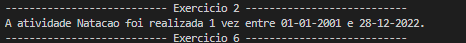
\includegraphics[width=1\linewidth]{rec1.png}  % largura percentual
\caption{Answer to problem 2}
\label{fig:ex2}
\end{figure}

\subsection{Exercício 3}
Para a resolução do exercício 3, é necessária , também, a função "ConvertToDate". Neste exercício, necessitamos da informação presente nos ficheiros de texto "praticantes" e "atividades", para listar os praticantes por ordem decrescente de número de participante, que realizaram uma atividade num período de tempo.

\begin{lstlisting}[caption=Exemplo exercício 3]
for (i = 0; i < atividadesLen; i++)
    {
        for (p = praticantesLen; p >= 0; p--)
        {
            if (strcmp(atividades[i].numPraticante, praticantes[p].numPraticante) == 0)
            {
                diaT = (atividades[i].data[0] - 48) * 10 + (atividades[i].data[1] - 48);
                mesT = (atividades[i].data[3] - 48) * 10 + (atividades[i].data[4] - 48);
                anoT = (atividades[i].data[6] - 48) * 1000 + (atividades[i].data[7] - 48) 
                * 100 + (atividades[i].data[8] - 48) * 10 + (atividades[i].data[9] - 48) * 1;
                if (anoT >= anoI && anoT <= anoF)
                {
                    totalT = convertToDate(diaT, mesT, anoT);
                    if (totalT >= totalI && totalT <= totalF)
                    {
                        printf("O praticante %s nº %s praticou %s no intervalo 
                        selecionado.\n", praticantes[p].nome, 
                        praticantes[p].numPraticante, atividades[i].nomeAtividade);
                    }
                }
            }
        }
    }
\end{lstlisting}

\begin{figure}[htbp]
\centering
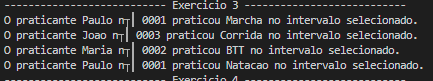
\includegraphics[width=1\linewidth]{rec2.png}  % largura percentual
\caption{Answer to problem 3}
\label{fig:ex3}
\end{figure}

\subsection{Exercício 4}
Para a resolução do exercício 4, é necessária a função "ConvertToDate". Neste exercício, necessitamos da informação presente no ficheiro de texto "planoAt", para apresentar o plano de atividades de determinado tipo.
A informação é pedida no ficheiro "Main.c", quando a função é chamada.

\begin{lstlisting}[caption=Exemplo exercício 4]
for (i = 0; i < planoLen; i++)
    {
        if (strcmp(plano[i].nomeAtividade, tipo) == 0)
        {
            diaI1 = (plano[i].dataInicio[0] - 48) * 10 + (plano[i].dataInicio[1] - 48);
            mesI1 = (plano[i].dataInicio[3] - 48) * 10 + (plano[i].dataInicio[4] - 48);
            anoI1 = (plano[i].dataInicio[6] - 48) * 1000 + (plano[i].dataInicio[7] - 48) 
            * 100 + (plano[i].dataInicio[8] - 48) * 10 + (plano[i].dataInicio[9] - 48) * 1;

            diaF1 = (plano[i].dataFim[0] - 48) * 10 + (plano[i].dataFim[1] - 48);
            mesF1 = (plano[i].dataFim[3] - 48) * 10 + (plano[i].dataFim[4] - 48);
            anoF1 = (plano[i].dataFim[6] - 48) * 1000 + (plano[i].dataFim[7] - 48) 
            * 100 + (plano[i].dataFim[8] - 48) * 10 + (plano[i].dataFim[9] - 48) * 1;

            if (anoI1 >= anoI && anoF1 <= anoF)
            {
                totalI1 = convertToDate(diaI1, mesI1, anoI1);
                totalF1 = convertToDate(diaF1, mesF1, anoF1);

                if (totalI <= totalI1 && totalF1 <= totalF)
                {
                    printf("%s foi praticado no intervalo %s - %s pelo praticante nº%s\n",
                    plano[i].nomeAtividade, dataI, dataF, plano[i].numPraticante);
                }
            }
        }
    }
\end{lstlisting}

\begin{figure}[htbp]
\centering
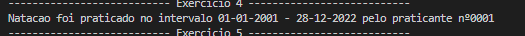
\includegraphics[width=1\linewidth]{rec3.png}  % largura percentual
\caption{Answer to problem 4}
\label{fig:ex4}
\end{figure}

\subsection{Exercício 5}
Para a resolução do exercício 5, necessitamos da informação presente nos ficheiros de texto "atividades" e "dados", para calcular a média dos tempos em que os praticantes estiveram envolvidos em atividades físicas. Para tal, é necessário os índices dos praticantes e das atividades, que irão ser comparados, assim como um contador. Será apresentado o tempo médio (em segundos) dos praticantes.

\begin{lstlisting}[caption=Exemplo exercício 5]
for (indiceP = 0; indiceP < praticantesLen; indiceP++)
    {
        // reiniciar os contadores
        ans = 0;
        counter = 0;
        // ver todas as atividades realizadas
        for (indiceA = 0; indiceA < atividadesLen; indiceA++)
        {
            // encontramos uma atividade praticada pelo praticante
            if (strcmp(praticantes[indiceP].numPraticante, 
            atividades[indiceA].numPraticante) == 0)
            {
                // contadores são incrementados
                ans += atividades[indiceA].duracao;
                counter++;
            }
        }
        printf("O praticante %s demorou cerca de %.2f segundos em média 
        por atividade.\n", praticantes[indiceP].nome, ans / counter);
    }
\end{lstlisting}

\begin{figure}[htbp]
\centering
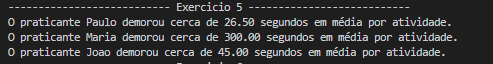
\includegraphics[width=1\linewidth]{rec4.png}  % largura percentual
\caption{Answer to problem 5}
\label{fig:ex5}
\end{figure}

\subsection{Exercício 6}
Para a resolução do exercício 6, necessitamos da informação presente nos ficheiros de texto "dados" e "planoAt", para gerar uma tabela de atividades planeadas e realizadas para todos os participantes.

\begin{lstlisting}[caption=Exemplo exercício 6]
// iterar pelo plano das atividades
    for (indiceA = 0; indiceA < planoLen; indiceA++)
    {
        // não sabemos o nome do praticante
        strcpy(nome, "");
        for (indiceP = 0; indiceP < praticantesLen; indiceP++)
        {
            // encontramos o praticante que queremos
            if (strcmp(planoAtividades[indiceA].numPraticante,
            praticantes[indiceP].numPraticante) == 0)
            {
                // guardamos o nome do praticante
                strcpy(nome, praticantes[indiceP].nome);
            }
        }
        // imprimir a linha da tabela
        printf("%s \t %s \t %s \t %s \t %s \t %d \t %s\n", 
        planoAtividades[indiceA].numPraticante, nome, planoAtividades[indiceA].nomeAtividade, planoAtividades[indiceA].dataInicio, planoAtividades[indiceA].dataFim, planoAtividades[indiceA].valor, planoAtividades[indiceA].unidade);
    }
\end{lstlisting}

\begin{figure}[htbp]
\centering
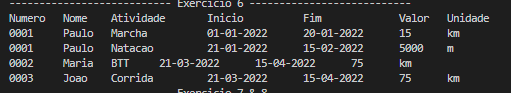
\includegraphics[width=1\linewidth]{rec5.png}  % largura percentual
\caption{Answer to problem 6}
\label{fig:ex6}
\end{figure}

\subsection{Exercícios 7 e 8}
Para a resolução do exercício 7 e 8, todos os ficheiros de texto serão necessários e será criado um ficheiro binário, para onde será transcrita a informação pedida.

\begin{lstlisting}[caption=Exemplo exercícios 7 e 8]
FILE *ex8 = fopen("ex8.bin", "w");
    if (ex == 7)
    {
        printf("Numero \t Nome \t Inicio \t Fim \t\t Total \t Tempo \t Dia D \t\n");
    }
    for (indicePlano = 0; indicePlano < planoLen; indicePlano++)
    {
        total = 0;
        tempo = 0;
        for (indicePac = 0; indicePac < praticantesLen; indicePac++)
        {
            if (strcmp(plano[indicePlano].numPraticante, praticantes[indicePac].numPraticante) == 0)
            {
                for (indiceAR = 0; indiceAR < atividadesLen; indiceAR++)
                {
                    // encontramos uma atividade realizada pelo praticante, que pertence ao plano
                    if (strcmp(atividades[indiceAR].numPraticante, praticantes[indicePac].numPraticante) == 0 && strcmp(atividades[indiceAR].nomeAtividade, plano[indicePlano].nomeAtividade) == 0)
                    {
                        total += atividades[indiceAR].valor;
                        // guardar a unidade do valor
                        strcpy(aux, atividades[indiceAR].unidade);
                        tempo += atividades[indiceAR].duracao;
                        // é o dia em que foi colocado mais esforço?
                        if (atividades[indiceAR].valor > maxVal)
                        {
                            maxVal = atividades[indiceAR].valor;
                            strcpy(maxData, atividades[indiceAR].data);
                        }
                    }
                }
                if (ex == 7)
                {
                    printf("%s \t %s \t %s \t %s \t %d%s \t %d \t %s \t\n", praticantes[indicePac].numPraticante, praticantes[indicePac].nome, plano[indicePlano].dataInicio, plano[indicePlano].dataFim, total, aux, tempo, maxData);
                }
                else
                {
                    fprintf(ex8, "%s \t %s \t %s \t %s \t %d%s \t %d \t %s \t\n", praticantes[indicePac].numPraticante, praticantes[indicePac].nome, plano[indicePlano].dataInicio, plano[indicePlano].dataFim, total, aux, tempo, maxData);
                }
            }
        }
    }
\end{lstlisting}

\begin{figure}[htbp]
\centering
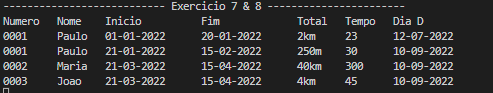
\includegraphics[width=1\linewidth]{rec6.png}  % largura percentual
\caption{Answer to problems 7 and 8}
\label{fig:ex78}
\end{figure}


	


\chapter{Conclusão}\label{chap:chap3}

Este projeto foi concluído com sucesso, apresentando uma avaliação \textbf{positiva}.

\textit{A aluna apresentou apenas alguns dos pontos mais importantes, tanto de Programação Imperativa, no que toca à apresentação do projeto, como de Laboratórios de Informática, no desenvolvimento do relatório, para o projeto não ficar demasiado extenso. Informação como tabelas, entre outros, não foram aqui demonstrados, pois não foi vista tal necessidade.} 
\include{chapter4}
\include{chapter5} 

%%----------------------------------------
%% Final materials
%%----------------------------------------

%% Bibliography
%% Comment the next command if BibTeX file not used, 
%% Assumes that bibliography is in ``myrefs.bib''
\PrintBib{myrefs}

%% Comment next 2 commands if numbered appendices are not used
\appendix
\include{appendix1}

%% Index
%% Uncomment next command if index is required, 
%% don't forget to run ``makeindex tese'' command
%\PrintIndex

\end{document}
